\subsection{Objetivos}
Este proyecto busca desarrollar un sistema desde el que se pueda gestionar un repositorio de árboles genealógicos y los usuarios del mismo sistema. El sistema tendrá que ser accesible a trabes de una API rest que permita a aplicaciones de terceros usar los datos del repositorio. Se ha establecido que el la persistencia de los árboles genealógicos tendrá que realizarse sobre una base de datos orientada a grafos, esta decisión se ha tomado para poder probar como una base de datos con estas características nos permite modelar un árbol genealógico aprovechando sus propiedades.\\
El modelo diseñado para la base de datos orientada a grafos para el almacenamiento de árboles genealógicos deberá ser  flexible (i.e. orientado a poder incluir nuevos atributos o conceptos manteniendo la consistencia del modelo) almacenar información genealógica y que este orientada a maximizar la eficiencia de las consultas más complejas que necesite ejecutar el sistema.\\
El objetivo de la API rest es cubrir todas las operaciones CRUD del repositorio y añadir funcionalidades extra sobre el sistema, las 2 funcionalidades estudiadas son la carga de archivos GEDCOM al repositorio y la búsqueda de personas similares entre los diferentes árboles almacenados.\\
La gestión de usuarios que realice la API rest se tendrá que realizar de forma segura para que los datos almacenados por los usuarios estén protegidos.

\subsection{Objetivos académicos}
Bajo los términos en los que se inscribió el proyecto los objetivos que este tendrá que alcanzar serán:

\begin{description}
	\item[CES1.1]:\\Desarrollar, mantener y evaluar sistemas y servicios software complejos o críticos.
	\item[CES1.2]:\\Dar solución a problemas de integración en función de las estrategias, de los estándares y tecnologías disponibles.
	\item[CES1.4]:\\Desarrollar, mantener y evaluar servicios y aplicaciones distribuidas con soporte de red.
	\item[CES1.5]:\\Especificar, diseñar y implementar bases de datos.
	\item[CES1.6]:\\Administrar bases de datos (CIS4.3)
	\item[CES1.9]:\\Demostrar comprensión en la gestión y gobierno de sistemas software.
	\item[CES2.2]:\\Diseñar soluciones apropiadas en uno o más dominós de la aplicación, usando métodos de ingeniería del software que integren aspectos éticos, sociales, legales y económicos. 
\end{description}

En las conclusiones de explicara como se han cumplido estos objetivos de forma detallada.


\subsection{Metodologia y rigor}
Las metodologías usadas son las siguientes:

\subsubsection{SCRUM}
Para el desarrollo del proyecto se ha escogido como metodología de trabajo SCRUM, los \textit{sprints} dado la naturaleza del proyecto se han adaptado esta metodología ágil para ser usada por una sola persona. La metodología de trabajo se ha definido de la siguiente forma:
\begin{description}
	\item[Product backlog]:
	\linebreak Para crear el \textit{product backlog} se han definido un seguido de historias de usuario, de acuerdo con el tutor del proyecto, que asume el rol de \textit{product owner}. Estas historias de usuario se revisaran constantemente en los \textit{sprint backlogs}.
	\item[Sprints]:
	\linebreak Se desarrollaran a lo largo de dos semanas, en este tiempo se desarrollaran las historias de usuario escogidas.
	\item[Sprint backlog]:
	\linebreak Se realizaran al final de cada \textit{sprint}, dado que esta tarea estará limitada por la disponibilidad del tutor y el alumno, se dara flexibilidad pudiendo realizar el \textit{sprint backlog} de varios \textit{sprints} en una reunión. Durante estas reuniones se revisaran las historias de usuario, reorganizando su prioridad, modificando su contenido, añadiendo nuevas o eliminando historias que no se crean necesarias.
	\item[Product owner]:
	\linebreak El \textit{product owner} es el responsable de de mantener el \textit{product backlog}, entre sus tareas asegurar el valor del trabajo realizado por el equipo de desarrollo, este rol lo asumirá el director del proyecto.
	\item[Scrum master]:
	\linebreak Es la persona responsable de asegurarse que la metodologia se sigue y es usada correctamente. Este rol se asumirá por el estudiante.
	\item[Equipo de desarrollo]:
	\linebreak Se encarga de desarrollar las funcionalidades del producto durante los \textit{sprints}, para este proyecto no se usara un equipo, el único desarrollador sera el estudiante.
\end{description}
En la figura \ref{fig:scrum} se puede ver un esquema de las fases de la metodologia.
\begin{figure}[ht!]
	\center
	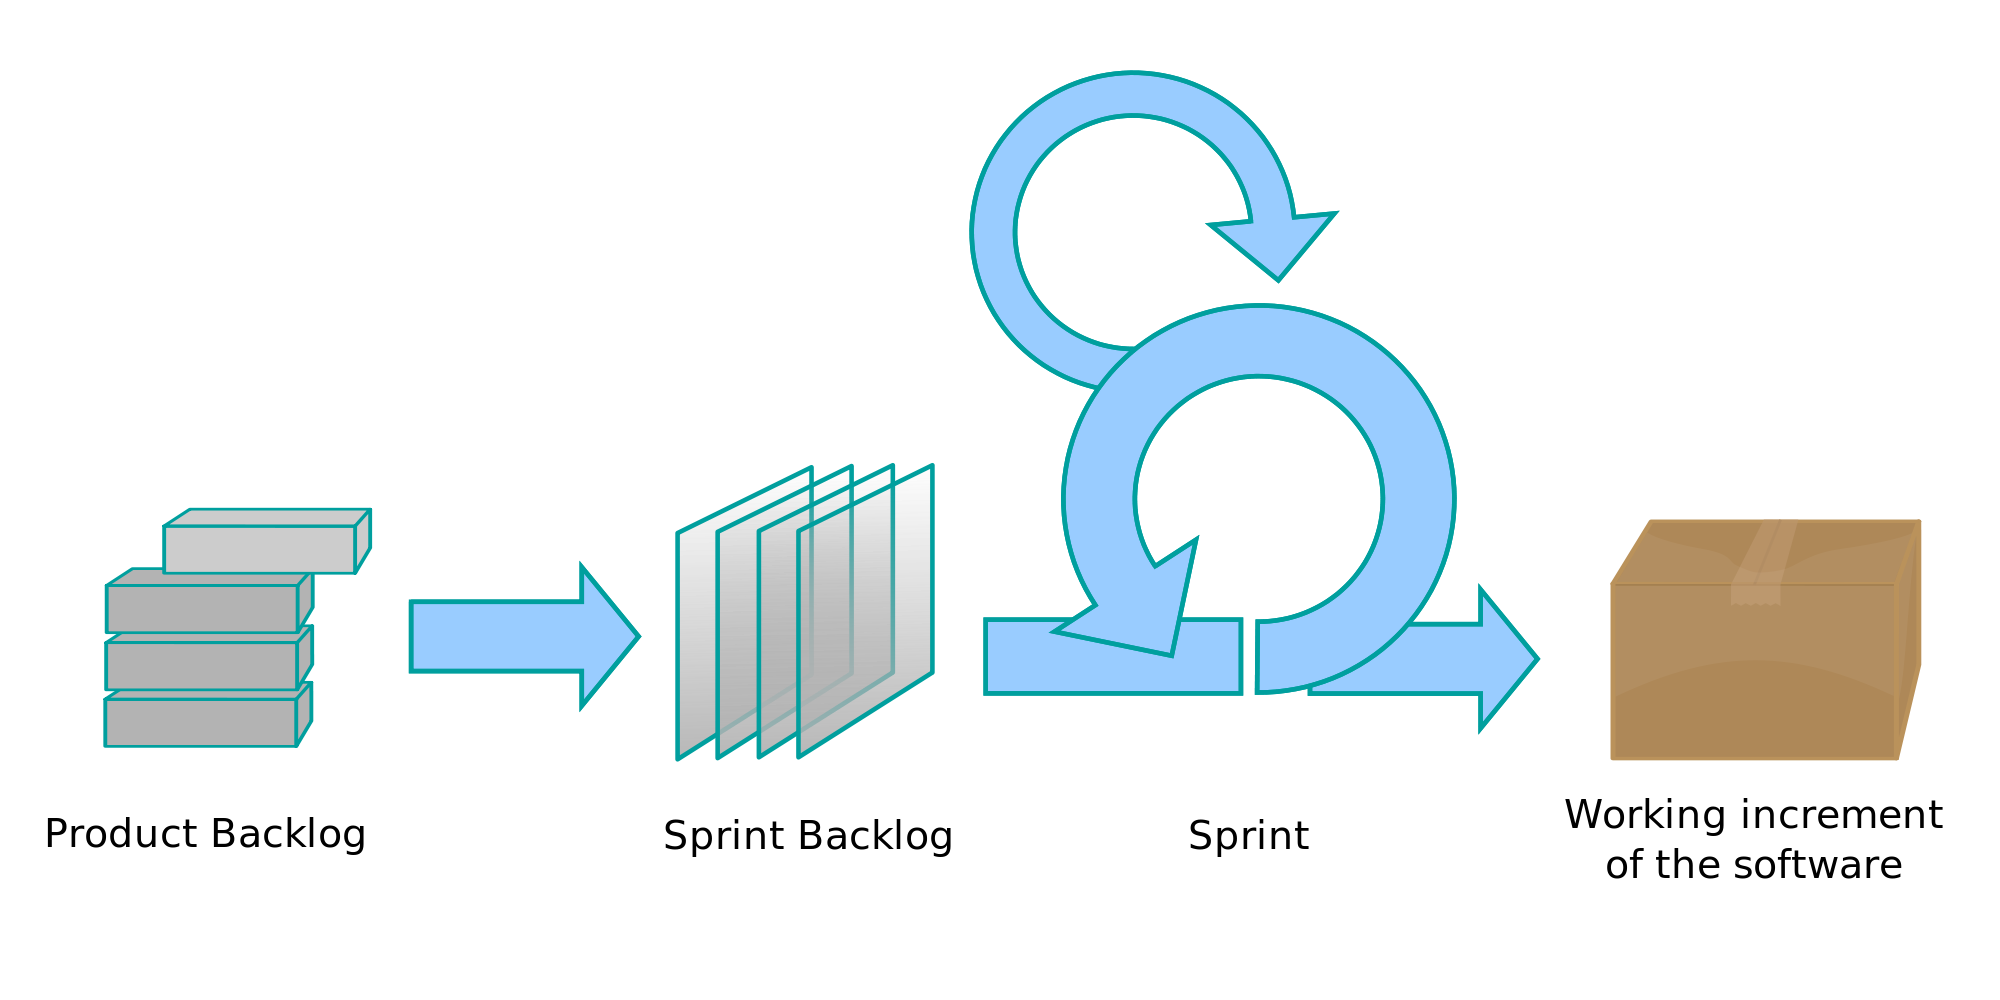
\includegraphics[scale=0.2]{Scrum_process.png}
	\caption{Metodología SCRUM}
	\label{fig:scrum}
\end{figure}

Finalmente si bien no podemos decir que la metodologia usada sea SCRUM, más bien una adaptación de esta metodologia a las necesidades del proyecto, para simplificar en el trabajo se hablara de esta adaptación como SCRUM, si bien sabiendo que es una adaptación de este.
\newpage
\subsection{Metodo de validación}
Al seguir la metodología Scrum, no se necesita definir criterios de aceptación de todo el proyecto entero, puesto que la propia dinámica ofrece un fuerte control del producto por parte del ``product owner''.
Uno de los mejores aspectos de esta metodología es la gran cohesión que crea entre todos los miembros involucrados al proyecto. En general siempre hay una misma visión del producto que se está creando, y el ``product owner'' puede ir perfilando el producto durante el transcurso de los sprints.
No se definen criterios de aceptación de todo el producto, pero si que se definen criterios de aceptación de las diferentes tareas. Gracias a que las tareas tienen una granularitat muy pequeña, los criterios de aceptación pueden ser muy precisos y concisos.
Cómo se ha visto anteriormente, los encargados de validar los criterios de aceptación de las tareas es el \textit{product owner}, durante los \textit{sprint backlogs}.

\subsection{Fases de desarrollo}
El desarrollo del sistema constara de cuatro fases, que se realizaran de manera secuencial de la siguiente manera.

\subsubsection{Análisis de requisitos y estudio previo}
Primero, durante el transcurso de GEP se realizara un estudio previo donde se definirá el estado del arte, alcance, planificación, se explicara la metodologia que se seguirá, también se realizara también una estimación de costes.

Después, En la primera etapa del proyecto se realizara el análisis de requisitos, mediante este análisis se describirán tanto los requisitos funcionales como no funcionales que tendrá que cubrir la solución que se desarrolle, por supuesto estos requisitos se revisaran y priorizaran según se vayan desarrollando \textit{sprint}.

\subsubsection{Especificación}
Una vez realizado el análisis de requisitos se definirá la especificación del proyecto. Con la especificación se definirán los casos de uso y un diagrama UML con nuestro modelo conceptual de datos.

\subsubsection{Diseño}
En la fase de diseño decidiremos que patrones aplicaremos en nuestro proyecto y estudiaremos como las tecnologías que se ha decidido usar ayudan a seguir ciertas arquitecturas. También se estudiaran los protocolos que se vayan a usar.\\
Por ultimo se definirá el diseño del modelo de datos establecido a partir de diseño del modelo conceptual de datos y se decidirán diferentes técnicas de optimización. También se estudiara el diseño de capa de domino y se definirán los diagramas de secuencia más importantes.

\subsubsection{Implementación y pruebas}
Durante la implementación se realizara el desarrollo del sistema,  teniendo en cuenta las decisiones que se hayan tomado durante las etapas anteriores. A medida que se vaya avanzando en la implementación se diseñaran test de integración par ir validando el desarrollo.

\subsection{Posibles obstáculos}

\paragraph{Tiempo:}
La gestión del tiempo sera uno de los obstáculos más notables a la hora de desarrollar el proyecto, dado que se pretende plantear un proyecto que no necesariamente ha de concluir su desarrollo con la entrega final, para ello se tendrán que plantear claramente las iteraciones necesarias para tener una versión funcional del software y el tiempo de desarrollo que requerirán.
\paragraph{Integración de tecnologías y desarrollo:}
Uno de los objetivos de este proyecto es combinar ciertas tecnologías con las que no se ha trabajado anteriormente, esto puede repercutir en que se encuentren dificultades al integrarlas. Por ello este hecho se tendrá que tener en cuenta en la planificación temporal.
